\section{Introduction}
\Title{Expected risk minimization}
We have a \textbf{data source} $\mathcal{X}$ from which we draw \textbf{samples} $X_1, \dots, X_n$. We can see $\mathcal{X}$ as a probability distribution. Define $\mathcal{H}$ as a class of \textbf{hypotheses} (possible explanations of $\mathcal{X}$). Want to select the one that best explains $\mathcal{X}$. \\
A \textbf{risk/loss function} $l : \mathcal{H} \times \mathcal{X} \rightarrow \R$ quantifies how well we think that a given hypothesis $H \in \mathcal{H}$ explains given data $X \in \mathcal{X}$. \\
The \textbf{expected risk} is $l(H) := \E_{\mathcal{X}}[l(H, X)]$. Goal: Find $H \in \mathcal{H}$ with the smallest expected risk: $H^* = \argmin_{H \in \mathcal{H}} l(H)$.
Problem: We do not know the distribution: we can only work with finitely many samples. We try to be \textbf{probably approximately correct (PAC)}: take tolerances $\delta, \epsilon > 0$, we want to produce a hypothesis $\Tilde{H} \in \mathcal{H}$ such that $l(\Tilde{H}) \leq \inf_{H \in \mathcal{H}}{l(H)} + \epsilon$.\\
\Title{Empirical risk minimization}
We have \textbf{training data} $X_1, \dots, X_n$ from which we compute the \textbf{empirical risk}: $l_n(H) = \frac{1}{n}\sum_{i=1}^n{l(H, X_i)}$ of a hypothesis $H$. For $n \rightarrow \infty$, this converges to $l(H)$. Formally the \textbf{weak law of large numbers} states, that for $H \in \mathcal{H}$ and $\delta, \epsilon > 0$ we have $n_0$ such that for $n_0 \geq n$ we have $\abs{l_n(H) - l(H)} \leq \epsilon$ with probability at least $1 - \delta$. \\
We use \textbf{empirical risk minimization} as a proxy for risk minimization: For $n \in \N$ and $X_1, \dots, X_n \sim \X$ produce a hypothesis $\Tilde{H}_n$ such that $l_n(\Tilde{H}_n) \leq \inf_{H \in \mathcal{H}}{l_n(H)} + \epsilon$. \\
\textbf{Careful:} Empirical risk does \textit{not} always converge to expected risk(!).
\Title{The map of learning}
\begin{wrapfigure}[18]{l}{0.12\textwidth}
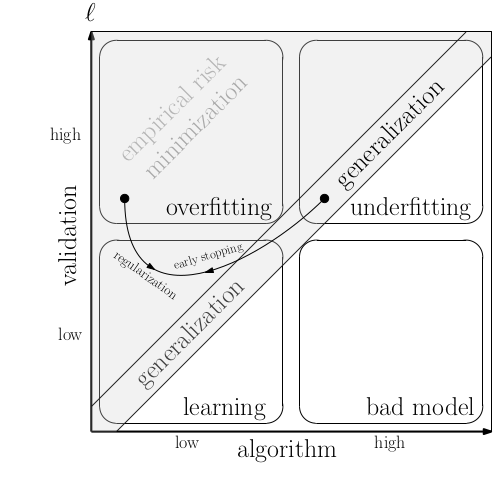
\includegraphics[scale=0.2]{ODS/images/map_of_learning.png}
\end{wrapfigure}
\textbf{Algorithm}: computational procedure according to which a hypothesis $H_n$ is obtained from training data $X_1, \dots, X_n$. \\
\textbf{Validation}: Once a hypothesis $H_n$ has been obtained through training, one also needs to assess its expected risk, i.e. locate $H_n$ in the $l$-dimension. Using the weak law of large numbers, $l(H_n)$ can be estimated via its empirical risk on test data—fresh samples from $\mathcal{X}$ that the algorithm has not seen. \\
\textbf{Overfitting}: If our learning algorithm returns a hypothesis with low empirical risk but high expected risk, we have a case of overfitting. The main cause of overfitting is that our theory (hypothesis class $\mathcal{H}$ and loss function $l$) is so complex that it allows us to almost perfectly explain any training data. \\
\textbf{Underfitting}: If the learning algorithm returns a hypothesis with high empirical risk, we cannot even explain the training data. In this case, there is no justified hope to be able to explain unseen data. The main cause of underfittting is that our theory is too simple to capture the nature of the data. \\
\textbf{Learning}: If both empirical and expected risk are low, we can make a case that we have learned something. \\
\textbf{Generalization}: Ideally, the expected risk is close to the empirical risk, and if this happens, we have generalization. This means that the hypothesis explains unseen data equally well as the training data. But it does \textit{not} mean that the explanation is good. \\
\textbf{Regularization}: In the case that overfitting is observed, a possible remedy is to add a regularization term $r$ to the loss function $l$ with the goal of \textit{punishing} complex hypotheses. Empirically minimizing $l' = l + \lambda r$ for a real number $\lambda > 0$ therefore has the effect that we introduce a \textbf{bias}, meaning that we deviate more and more from our theory, with the effect that the empirical risk increases. But as the intended consequence, the \textbf{variance} (sensitivity to the training data) decreases, and this may reduce the expected risk. \\
\Title{Worst-case versus average-case complexity} 
The classical measure of algorithm performance is its \textbf{worst-case complexity}, the function that maps $n$ to the maximum runtime of the algorithm over all possible inputs of size $n$. The \textbf{average case complexity} is the function that maps $n$ to the expected runtime of the algorithm, taken over its input distribution. \\
\Title{The estimation-optimization tradeoff} 
As we inevitably lose precision in going from empirical to expected risk, it doesn’t help to optimize the empirical risk to a significantly higher precision. Let us call the precision that we lose in going from empirical to expected risk the \textbf{estimation error}; the precision we lose in finding only an almost best explanation of the training data is the \textbf{optimization error}. In small-scale learning, it doesn’t hurt to go for as small an optimization error as we can. But in large-scale learning, we may need to give up on some optimization precision in order to be able to stay within the optimization time budget. The \textbf{estimation-optimization tradeoff} consists in finding the most efficient way of spending the resources under the given constraints.